% !TEX root = ../../main.tex
\section{Change Detection}\label{sec:method_change_detection}
In the following sections we haved discussed what data is used for the model construction how the model is interpreted in the context of change detection.
In this section we discuss the methods applicable to the extracted radius $R$ of the hypersphere, in order to indicate a change in the underlying distribution properties.
This employs the second stage of our algorithm, analogue to the second stage of the unifying framework by Takeuchi and Yamanishi~\cite{takeuchi2006unifying}.

In the previous sections we have discussed how a multi-dimensional signal can be reduced to a single dimension time series data based on the radius $R$.
We have argued that in the case of a change in the underlying data, where it becomes more heterogeneous, we expect an increase in the radius $R$.
In the same manner we expect that when the change is in the oldest data objects of the working set the radius $R$ will decrease, since the data becomes more homogeneous.
An abstract representation of these expectations is illustrated in Figure~\ref{fig:radius_expectation}.

\begin{figure}
  \centering
    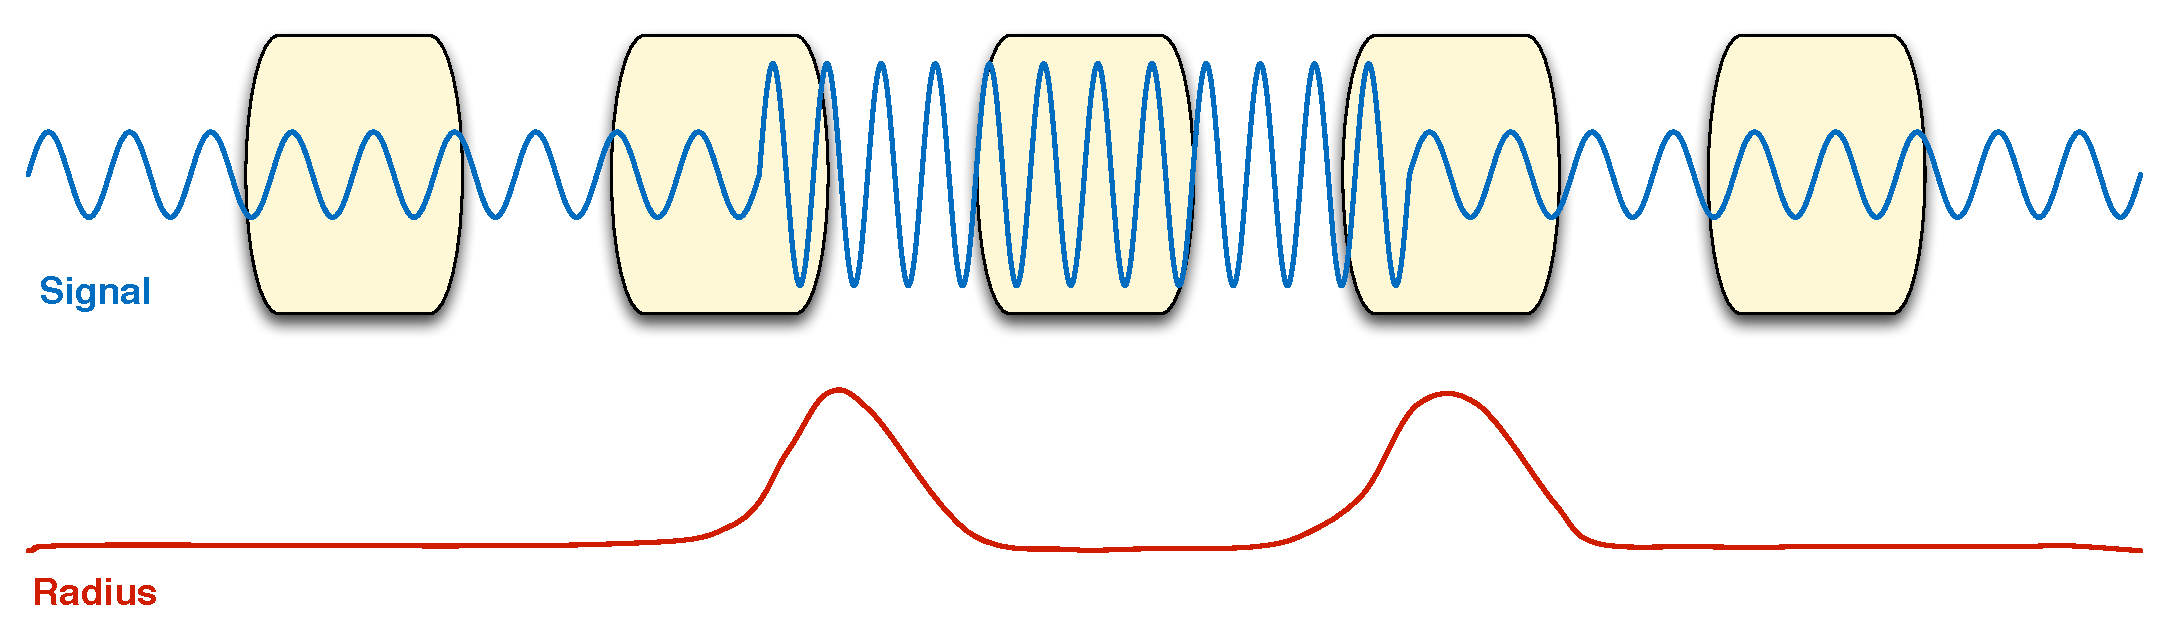
\includegraphics[width=\textwidth,height=\textheight,keepaspectratio]{./Figures/chapter4/expected_behaviour.pdf}
  \caption[Expected radius behavior]{Expected behavior of the radius $R$ of the hypersphere. The upper part shows a typical sinusoidal time series signal. The lower graph visualizes an abstract expectation of the values of $R$. Five possible windows are illustrated. The left, middle, and right windows cover an area of homogeneous signal. The expected value of $R$ is low. The other two windows cover a change entering and leaving the window, respectively. At these locations the radius $R$ is expected to increase temporarily.}
  \label{fig:radius_expectation}
\end{figure}

The problem of change detection in complex multi-dimensional time series is now reduced to finding change in a one-dimensional time series.
Besides the dimensionality reduction, the form of the signal is also simplified.
Whereas the original signal was represented as a sinusoidal or second order \gls{ar} model, the new time series is of much simpler form.
In our method we leave open the precise method which is used to find change points in the obtained change indication values.
Below, we will gives two examples of methods which can be applied.
The first is a family of methods based on the \gls{cusum} method.
The second example is a ratio-based thresholding mechanism used by Camci~\cite{camci2010change}.
We conclude this section by discussing some post-processing techniques we have used, to decrease the number of false positives.

\subsection{CUSUM based methods}
Many of the simple change detection methods are based on \gls{cusum}, originally introduced by Page~\cite{page1954continuous}.
Many variations and extensions of the method are proposed and used (\cite{inclan1994use,alippi2006adaptive,hsu2007mosum}).
Here we will discuss the simple form, which only detects changes for an increase of the examples, in this case the radius $R$.
The cumulative sum for all the values is calculated:
\begin{equation}
  S_n = \sum_{k=1}^n r_k
\end{equation}
and a change is detected when the value of the cumulative sums minus the minimum encountered exceeds a predetermined threshold $h$:
\begin{equation}
  S_n - \operatorname*{min}_{0 \le i < n} S_i \ge h.
\end{equation}

Extensions of the \gls{cusum} method have been proposed.
Amongst others, extensions which extend its use to two-threshold methods, and methods appropiate for changes in mean or variance \cite{inclan1994use}.
Whilst adaptive methods have been proposed \cite{alippi2006adaptive}, most methods require manual determination of the threshold parameter $h$.

\subsection{Ratio-thresholding}
The second example of an algorithm that interprets the change indication time series and transforms it to change detection is the radius ratio thresholding method used by Camci~\cite{camci2010change}.
The method shares characteristics with \gls{cusum}, since it relies on summation of historic data and thresholds for change detection.
The method calculates the radius ratio $\hbar_t$ by taking the ratio of the current radius $r_t$ at time $t$ to the average radii since the last change point $y$:
\begin{equation}\label{eq:ratio_radius}
  \hbar_t = \frac{r_t}{\operatorname*{mean}(r_{y:t-1})},
\end{equation}
where $\operatorname*{mean}(r_{y:t-1})$ is the average of the previous approximated radii.
By using only historic data, this method can be incorporated in an online change detection method.
The ratio $\hbar_t$ is compared with two thresholds: the low threshold $th_\text{low}$ and the high threshold $th_\text{high}$.
When the data objects in the working set becomes more homogeneous at time $t$, the radius $R$ of the hypersphere and thereby the ratio $\hbar_t$ will decrease.
When the new value of $\hbar_r$ is lower than the low threshold $th_\text{low}$, a change detection is observed for time $t$.
The same holds for a more heterogeneous set of data and an increase of $\hbar_r$ higher than $th_\text{high}$.

The appropriate values for the thresholds are highly depended on the characteristics of the data and the trade-off parameter $C$ (as discussed in Section~\ref{subsec:oc-svm-svdd}).
This trade-off parameters regulates the fraction of data objects that will be rejected from the constructed model.
Since a high value of $C$ assigns a high penalty to outliers, data objects are more likely to be incorporated into the hypersphere by increasing the radius.
For low values of $C$ the cost of rejecting data objects is, compared to the benefits of a smaller hypersphere, relatively low.
This gives a relation between the parameters $C$, $th_\text{low}$, and $th_\text{high}$ and the sensitivity of the radius ratio based thresholding method.
A high value of $C$, or values close to $1$ for $th_\text{low}$ and $th_\text{high}$ result in a sensitive change detection procedure.
The reverse results in less sensitive methods.
The correct values for the intended sensitivity need to be empirically determined.

\subsection{Post-processing}
In our method we use the ratio based thresholding, since it is also used by Camci~\cite{camci2010change}.
From preliminary experiments we observed that a single change in the data can cause many detected change points, using the ratio based method.
This phenomenon can be explained by the nature of the thresholding method.
Since a single (high or low) threshold is set for ratio of the radii, high values are considered to be a change point before the highest point of the peak.
As illustrated in Figure~\ref{fig:tresholding}, the peak at $t_1$ represents a single change point.
The region from $t_2$ to $t_3$ is strictly increasing.
At $t_2$ a change point is detected, since $\hbar_t$ exceeds the threshold.
But since it is increasing up to $t_3$, all values of $\hbar_t$ in that period will trigger the ratio based method to indicate a change point.

To overcome this problem, we apply a post-processing method on the generated change points.
All the change points that are within a time period $\delta$ of each other are merged together.
\TODO{Merged to the front, or to the back, depending on high/low threshold exceeding?}

\begin{figure}
  \centering
    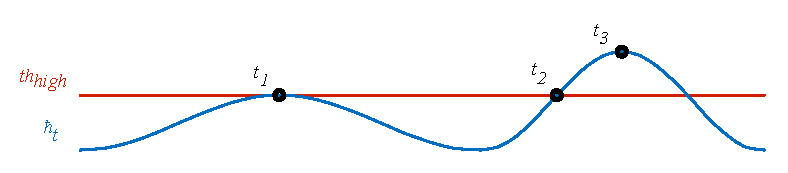
\includegraphics[width=\textwidth,height=\textheight,keepaspectratio]{./Figures/chapter4/signal_threshold.pdf}
  \caption[Thresholding]{Abstract illustration of the radius ratio thresholding. The peak at $t_1$ generates a single change point. The region between $t_2$ and $t_3$ generates multiple change points, since the value of $\hbar_t$ keeps increasing.}
  \label{fig:tresholding}
\end{figure}